\documentclass[border=5mm, convert]{standalone}
\usepackage{tikz}
\usetikzlibrary{shapes,arrows}
\usetikzlibrary{matrix,arrows.meta,positioning}

\begin{document}
% \tikzstyle{arrow} = [thick,->,>=stealth]
% \tikzstyle{box} = [rectangle, 
% minimum width=0.5cm, 
% minimum height=1cm,
% text centered, 
% draw=black,text width=2cm]
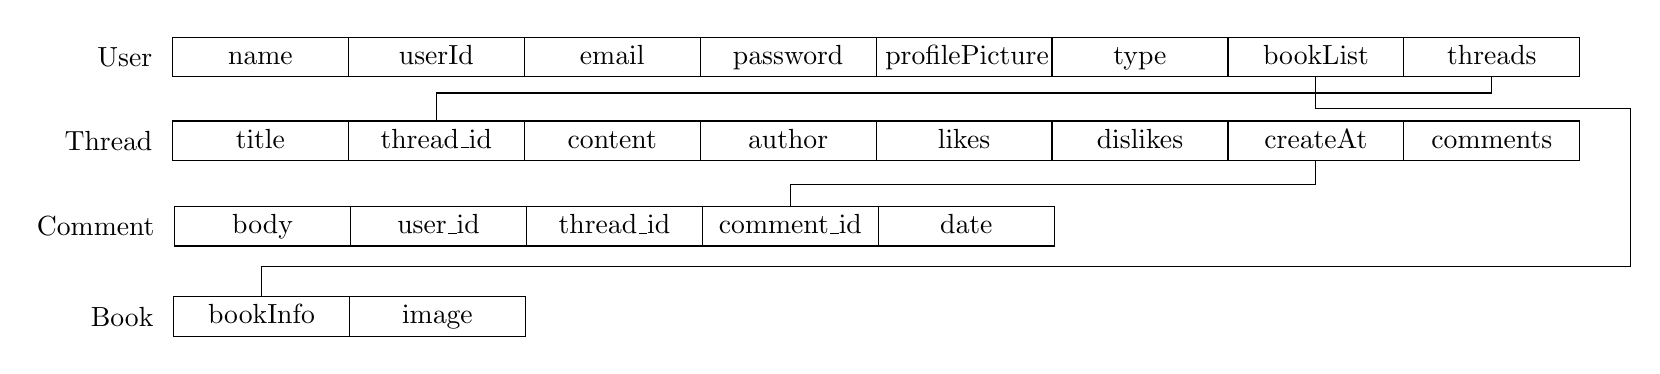
\begin{tikzpicture}[
    table/.style={
        matrix of nodes, 
        % nodes in empty cells, 
        column sep=-\pgflinewidth, 
        row sep=-\pgflinewidth, 
        nodes={
            text centered,
            draw,
            % minimum width=1.7cm, 
            text width=2cm,
            text height=1.5ex,
            text depth=.25ex
        }, 
        row 1/.style={nodes={}}
    }]
    
    \matrix(User) [table, label=left:User] {
        name & userId & email & password & profilePicture & type & bookList & threads & \\};
    
    \matrix(Thread) [table, label=left:Thread, below=0.3cm of User] {
        title & thread\_id & content & author & likes & dislikes & createAt & comments & \\};
    
    \matrix(Comment) [table, label=left:Comment, below=0.45cm of Thread-1-3] {
        body & user\_id & thread\_id & comment\_id & date & & & &\\};
    
    \matrix(Book) [table, label=left:Book, below=1.95cm of Thread-1-1.5] {
        bookInfo & image & \\};
    
    \draw (User-1-8.south)--++(0,-.2)-|(Thread-1-2);
    \draw (Thread-1-7.south)--++(0,-.3) -| (Comment-1-4.north);
    \draw (User-1-7.south) |- ++(0,-.4) -| ++(4.0,0) |-  ++(0,-2.0) -| ++(0,0) -| (Book-1-1.north);
    % \draw (Course-2-1.south)--++(0,-.5)-|(Student-2-3.south);
    \end{tikzpicture}
\end{document}